\documentclass[11pt,a4paper]{article}
\usepackage[utf8]{inputenc}
\usepackage[T1]{fontenc}
\usepackage{lmodern}
\usepackage{amsmath,amssymb,mathtools}
\usepackage{bm}
\usepackage{booktabs}
\usepackage{longtable}
\usepackage{array}
\usepackage{enumitem}
\usepackage[margin=2.2cm]{geometry}
\usepackage{xcolor}
\usepackage{listings}
\usepackage{graphicx}
\usepackage[section]{placeins}
\graphicspath{{images/}}
\usepackage[colorlinks=true,linkcolor=blue!60!black,urlcolor=blue!60!black]{hyperref}
\usepackage[nameinlink]{cleveref}

\newcommand{\Om}{\hat{\Omega}}
\newcommand{\dd}{\mathrm{d}}
\newcommand{\kron}{\otimes}
\newcommand{\Lmax}{\Lambda}
\newcommand{\R}{\mathbb{R}}
\newcommand{\pp}{{\bm{p}^{+}}}
\newcommand{\pmn}{{\bm{p}^{-}}}
\newcommand{\diag}{\operatorname{diag}}
\newcommand{\code}[1]{\texttt{#1}}

\lstset{language=Python,basicstyle=\ttfamily\small,columns=fullflexible,keepspaces=true,
        commentstyle=\color{black!55},keywordstyle=\color{blue!50!black},frame=single,framerule=0.3pt,
        xleftmargin=4pt,xrightmargin=4pt,showstringspaces=false}

\title{TT-Neutron-Transport\\[2pt]\large Theory and documentation of \texttt{SlabTransport}}
\date{2026-10-19}

\begin{document}
\maketitle
\sloppy
\tableofcontents

%==========================================================================================
\section{Theory}
\label{sec:theory}
%==========================================================================================

\subsection{Problem statement}
\label{sec:problem}

Slab $z\in[0,L]$, laterally infinite, full angular dependence $\Om=\Om(\mu,\varphi)$, $\mu=\Om\cdot\hat z$, energy groups $g=1,\dots,G$ ($g=1$ the fastest), time $t\in(0,T]$. The multigroup transport equation for the angular flux $\psi_g(z,\Om,t)$ is
\begin{equation}
\Big(\frac{1}{v_g}\partial_t+\mu\,\partial_z+\sigma_{t,g}(z)\Big)\psi_g
=\sum_{g'=1}^{G}\int_{4\pi}\sigma_{s,g'\to g}(z,\Om\cdot\Om')\,\psi_{g'}(z,\Om',t)\,\dd\Om'+Q_g(z,\Om,t),
\label{eq:transport}
\end{equation}
with inflow on the incoming half ranges and an initial condition,
\begin{equation}
\psi_g(0,\Om,t)=\psi^{\mathrm L}_g(\Om,t)\ \ (\mu>0),\qquad
\psi_g(L,\Om,t)=\psi^{\mathrm R}_g(\Om,t)\ \ (\mu<0),\qquad
\psi_g(z,\Om,0)=\psi^{0}_g(z,\Om).
\end{equation}
The steady-state problem drops $\partial_t$ and the initial condition.

\paragraph{Materials.} The slab is made of $C$ materials with constant data $\sigma^c_{t,g}$, $\sigma^{c}_{s,g'\to g}$. The material map $c(z)$ is piecewise constant, so
\begin{equation}
    \sigma_{t,g}(z)=\sum_{c=1}^{C}\mathbf{1}_c(z)\,\sigma^c_{t,g},\qquad
    \sigma_{s,g'\to g}(z,\cdot)=\sum_{c=1}^{C}\mathbf{1}_c(z)\,\sigma^c_{s,g'\to g}(\cdot).
\label{eq:materials}
\end{equation}

\paragraph{Scattering kernel.} Each material's kernel is expanded in Legendre polynomials up to $\Lmax$, and the addition theorem is used with the real orthonormal spherical harmonics $Y_{lm}(\Om)=A_{lm}(\mu)\Pi_m(\varphi)$:
\begin{gather}
\sigma^c_{s,g'\to g}(\mu_0)=\sum_{l=0}^{\Lmax}\frac{2l+1}{4\pi}\,\sigma^{l,c}_{s,g'\to g}P_l(\mu_0)
=\sum_{l=0}^{\Lmax}\sigma^{l,c}_{s,g'\to g}\sum_{m=-l}^{l}Y_{lm}(\Om)Y_{lm}(\Om'),\qquad \mu_0=\Om\cdot\Om',
\label{eq:kernel}\\
A_{lm}(\mu)=\sqrt{\tfrac{2l+1}{4\pi}\tfrac{(l-|m|)!}{(l+|m|)!}}\,P_l^{|m|}(\mu),\qquad
\Pi_m(\varphi)=\begin{cases}\sqrt2\cos(m\varphi)&m>0\\1&m=0\\\sqrt2\sin(|m|\varphi)&m<0\end{cases}
\end{gather}
The moments $\sigma^{l,c}_{s,g'\to g}=2\pi\int_{-1}^1\sigma^c_{s,g'\to g}(\mu_0)P_l(\mu_0)\,\dd\mu_0$ carry no $(2l+1)$ factor (OpenMC convention). Energy enters only through the matrices $\Sigma^{l,c}=[\sigma^{l,c}_{s,g'\to g}]_{gg'}$ (row $g$ receiving).

\paragraph{Azimuthal symmetry.} If $Q$, $\psi^0$ and the inflow do not depend on $\varphi$, neither does $\psi$, and only the $m=0$ terms of \eqref{eq:kernel} act on it.

%------------------------------------------------------------------------------------------
\subsection{Phase-space discretization}
\label{sec:discretization}

\begin{center}\small
\begin{tabular}{@{}lll@{}}
\toprule
index & range & meaning\\
\midrule
$i$ & $1,\dots,N_z$ & cell $K_i=[z_{i-1/2},z_{i+1/2}]$, $h=L/N_z$\\
$a,b$ & $0,\dots,p$ & Legendre mode in a cell; $s=(i,a)$, $N_s=N_z(p+1)$, mode index fastest\\
$n$ & $1,\dots,N_\mu$ & polar ordinate $\mu_n$\\
$q$ & $1,\dots,N_\varphi$ & azimuthal ordinate $\varphi_q$\\
$g$ & $1,\dots,G$ & energy group\\
$k$ & $1,\dots,N_t$ & time step, $t_k=k\Delta t$, $\Delta t=T/N_t$\\
$l$ & $0,\dots,\Lmax$ & Legendre order of the kernel\\
$c$ & $1,\dots,C$ & material\\
\bottomrule
\end{tabular}
\end{center}

\paragraph{Angle: discrete ordinates.} Product quadrature $\Om_{nq}=\Om(\mu_n,\varphi_q)$: $(\mu_n,w_n)$ the $N_\mu$-point Gauss--Legendre rule ($\sum_nw_n=2$; even $N_\mu$, so no $\mu_n=0$), $\varphi_q=2\pi(q-1)/N_\varphi$ with $w_q=2\pi/N_\varphi$. The rule integrates $Y_{lm}Y_{l'm'}$, $l,l'\le\Lmax$, exactly if $N_\mu\ge\Lmax+1$ and $N_\varphi\ge2\Lmax+1$. With azimuthal symmetry $N_\varphi=1$, $\varphi_1=0$, $w_1=2\pi$. Write $\mu_n^\pm=\max/\min(\mu_n,0)$, so $\mu_n=\mu^+_n+\mu^-_n$. The discrete kernel of order $l$ is the matrix over $(n,q)$
\begin{equation}
(K_l)_{(nq),(n'q')}=\sum_{m=-l}^{l}Y_{lm}(\Om_{nq})Y_{lm}(\Om_{n'q'})\,w_{n'}w_{q'}
=\sum_{m=-l}^{l}\big(\bm a_{lm}\bm a_{lm}^{\!\top}W_\mu\big)\kron\big(\bm\pi_m\bm\pi_m^{\!\top}W_\varphi\big),
\label{eq:Kl}
\end{equation}
with $\bm a_{lm}=(A_{lm}(\mu_n))_n$, $\bm\pi_m=(\Pi_m(\varphi_q))_q$, $W_\mu=\diag(w_n)$, $W_\varphi=\diag(w_q)$: a two-core TT matrix with $\mu|\varphi$ rank $2l+1$, or $1$ with azimuthal symmetry (only $m=0$, $\bm\pi_0\bm\pi_0^{\!\top}W_\varphi=[2\pi]$).

\paragraph{Space: upwind discontinuous Galerkin.} Upwind DG as introduced by Reed and Hill~\cite{ReedHill}. In $K_i$, $z=z_i+\frac h2\xi$, $\psi\approx\sum_{b=0}^p\psi_{ib}P_b(\xi)$. Testing with $P_a$ needs
\begin{gather}
M_h=\diag\Big(\frac{h}{2a+1}\Big),\qquad
S_{ab}=\int_{-1}^1P_bP_a'\,\dd\xi=\begin{cases}2&a>b,\ a+b\text{ odd}\\0&\text{else}\end{cases},\\
\pp=(P_a(1))_a=\bm 1,\qquad \pmn=(P_a(-1))_a=((-1)^a)_a .
\end{gather}
Integration by parts with upwind traces ($\psi^*_{i+1/2}$ from cell $i$ if $\mu>0$, from cell $i+1$ if $\mu<0$) gives, for cell $i$ and ordinate $n$,
\begin{equation}
\mu_n^+\big(\pp\pp^{\!\top}\bm\psi_i-\pmn\pp^{\!\top}\bm\psi_{i-1}\big)
+\mu_n^-\big(\pp\pmn^{\!\top}\bm\psi_{i+1}-\pmn\pmn^{\!\top}\bm\psi_i\big)-\mu_nS\bm\psi_i .
\end{equation}
On the boundary cells the missing neighbour is replaced by the inflow, which moves to the right-hand side as $\bm f^{\mathrm L}=\mu_n^+\psi^{\mathrm L}\pmn$ (cell $1$) and $\bm f^{\mathrm R}=-\mu^-_n\psi^{\mathrm R}\pp$ (cell $N_z$). Assembled over cells, with $E^\mp = \delta_{i,i\mp 1}$ the lower/upper shift matrices,
\begin{gather}
M=I_{N_z}\kron M_h,\qquad \mathsf S=I_{N_z}\kron S,\\
U^+=I_{N_z}\kron\pp\pp^{\!\top}-E^-\kron\pmn\pp^{\!\top},\qquad
U^-=E^+\kron\pp\pmn^{\!\top}-I_{N_z}\kron\pmn\pmn^{\!\top}.
\end{gather}
Sources and initial data enter as load vectors $(\bm f)_{(i,a)}=\int_{K_i}f(z)P_a\,\dd z$ ($=M$ times their Legendre coefficients).

\paragraph{Material masks.} Material interfaces lie on cell edges, so each cell has one material. With the one-hot map $\chi \in R^{N_z\times C}$ $\chi_{ic}=1$ if $K_i\subset c$, the cross sections are constant per cell, $\sigma_{t,g,i}=\sum_c\chi_{ic}\sigma^c_{t,g}$, and the reaction and scattering terms of cell $i$ are $\sigma^cM_h$. Over all cells this is the \emph{masked mass matrix}
\begin{equation}
M_c=\diag(\chi_{:c})\kron M_h,\qquad \sum_{c=1}^CM_c=M .
\label{eq:Mc}
\end{equation}
A homogeneous slab is $C=1$, $\chi=\bm 1$, $M_1=M$. Each row of $\chi$ has exactly one nonzero entry (no overlapping materials, no empty cells). A material boundary inside a cell would instead need full weighted mass matrices $\int_{K_i\cap c}P_aP_b\,\dd z$.

\paragraph{Time: backward Euler, all at once.} $\dot{\bm\psi}(t_k)\approx(\bm\psi^k-\bm\psi^{k-1})/\Delta t$, every other term at $t_k$. All $N_t$ steps are unknowns of one system; the coupling to the previous step is the matrix $D_t=\Delta t^{-1}(I-E^-)$ over $k$, and the known $\bm\psi^0$ moves to the right-hand side at $k=1$. In steady state $N_t=1$ and the time term is absent.

%------------------------------------------------------------------------------------------
\subsection{TT operator}
\label{sec:operator}

The unknown is a 5-dimensional tensor of DG modal coefficients $\Psi(s,n,q,g,k)$, stored as a TT with cores in the order $(s,n,q,g,k)$. Every term of the discrete system is a Kronecker product (or a short sum of them) in this order, with $V=\diag(v_g)$, $\Sigma^c_t=\diag(\sigma^c_{t,g})$, $D_\mu^{(\pm)}=\diag(\mu_n^{(\pm)})$:
\begin{equation}
\boxed{
\begin{aligned}
\mathcal A={}&\sum_{c=1}^{C}M_c\kron I\kron I\kron\Sigma^c_t\kron I &&\text{collision}\\
&+M\kron I\kron I\kron V^{-1}\kron D_t &&\text{time derivative}\\
&-\mathsf S\kron D_\mu\kron I\kron I\kron I+U^+\kron D_\mu^+\kron I\kron I\kron I+U^-\kron D_\mu^-\kron I\kron I\kron I &&\text{streaming}\\
&-\sum_{c=1}^{C}\sum_{l=0}^{\Lmax}M_c\kron K_l\kron\Sigma^{l,c}\kron I &&\text{scattering}
\end{aligned}}
\label{eq:A}
\end{equation}
where $K_l$ occupies the two angular slots. The discrete system is $\mathcal A\Psi=F$,
\begin{equation}
F=F_Q+F_0+F_{\mathrm L}+F_{\mathrm R},\qquad
\begin{aligned}
F_Q&=\bm Q_z\kron\bm Q_\mu\kron\bm Q_\varphi\kron\bm Q_E\kron\bm Q_t,\\
F_0&=\Delta t^{-1}\,\bm\Psi^0_z\kron\bm\Psi^0_\mu\kron\bm\Psi^0_\varphi\kron V^{-1}\bm\Psi^0_E\kron\bm e_1,\\
F_{\mathrm L}&=(\bm e_1\kron\pmn)\kron D^+_\mu\bm b^{\mathrm L}_\mu\kron\bm b^{\mathrm L}_\varphi\kron\bm b^{\mathrm L}_E\kron\bm b^{\mathrm L}_t,\\
F_{\mathrm R}&=(\bm e_{N_z}\kron\pp)\kron(-D^-_\mu)\bm b^{\mathrm R}_\mu\kron\bm b^{\mathrm R}_\varphi\kron\bm b^{\mathrm R}_E\kron\bm b^{\mathrm R}_t,
\end{aligned}
\label{eq:F}
\end{equation}
for separable data (subscripts = factors on the grids, $z$ factors as load vectors); sums of separable terms are sums of such vectors. The system is solved with AMEn. The solution is returned as modal coefficients; point values follow by contracting the space core with $P_a(\xi_r)$ at $N_{\mathrm{rec}}$ Gauss points per cell, and the scalar flux $\phi_g=\sum_{nq}w_nw_q\psi_g(\Om_{nq})$ by contracting the angular cores with their weights, without leaving the TT format.

\paragraph{Ranks of $\mathcal A$.} Grouped by the space factor, $\mathcal A=\sum_cM_c\kron\mathcal R_c+(U^+-\mathsf S)\kron D^+_\mu\kron\cdots+(U^--\mathsf S)\kron D^-_\mu\kron\cdots$, where $\mathcal R_c$ collects everything multiplying material $c$ (the time term joins through $M=\sum_cM_c$). The $M_c$ have disjoint supports, so
\begin{gather}
r_{z|\mu}=\dim\operatorname{span}\{\mathcal R_c\}+2\le C+2,\qquad r_{g|t}\le2\ (1\text{ steady}),\\
r_{\mu|\varphi}\le Cr_K+C+1,\qquad r_{\varphi|g}\le C(\Lmax+1)+C+1,
\end{gather}
with $r_K=(\Lmax+1)(\Lmax+2)/2$ ($\Lmax+1$ with azimuthal symmetry). The material index created in the space core is consumed only in the energy core, so it is carried through the angular cores. Equal materials share a column of $\chi$; affine combinations of other materials add nothing. Assembled term by term the first rank is $2C+3$; one TT rounding of $\mathcal A$ brings it to $C+2$. Example: graphite slab with a He-3 region, $P_{20}$, $G=128$, azimuthal symmetry: ranks $[3,23,23,1]$ for $C=1$, $[4,45,45,1]$ for $C=2$.

\paragraph{Inner product.} With $\Psi$ in modal coefficients and $F$ in load vectors, the Euclidean product over $s$ is the exact $z$ integral; angle uses the $S_N$ weights and time the rectangle rule:
\begin{equation}
\langle\psi,f\rangle\approx w_t\,\Psi\cdot(WF),\qquad W=I\kron W_\mu\kron W_\varphi\kron I\kron I,\qquad w_t=\Delta t\ (1\text{ steady}),
\label{eq:inner}
\end{equation}
one \code{tntt.dot} with the weights multiplied into the $\mu$ and $\varphi$ cores.

%------------------------------------------------------------------------------------------
\subsection{Adjoint problem}
\label{sec:adjoint}

\paragraph{Adjoint equation.} For a response $R$ of the forward solution, the adjoint flux $\psi^\dagger$ solves
\begin{equation}
\Big(-\frac{1}{v_g}\partial_t-\mu\,\partial_z+\sigma_{t,g}(z)\Big)\psi^\dagger_g
-\sum_{g'}\int_{4\pi}\sigma_{s,g\to g'}(z,\Om\cdot\Om')\,\psi^\dagger_{g'}\,\dd\Om'=q^\dagger_g(z,\Om,t),
\label{eq:adjoint}
\end{equation}
backward in time and along $-\Om$, with the group transfer transposed, $\Sigma^{l,c}\to(\Sigma^{l,c})^{\!\top}$ in every material; the angular kernel is symmetric and unchanged. Boundary and final conditions:
\begin{gather}
\psi^\dagger_g(0,\mu<0,t)=0,\qquad\psi^\dagger_g(L,\mu>0,t)=0,\notag\\
\psi^\dagger_g(z,\Om,T)=\begin{cases}0,&R=\int_0^T\langle q^\dagger,\psi\rangle\,\dd t,\\ v_g\,r_g(z,\Om),&R=\langle r,\psi(T)\rangle\ \ (q^\dagger=0).\end{cases}
\label{eq:adjoint-bc}
\end{gather}
The vacuum conditions hold only on the adjoint-incoming half ranges; the other halves are part of the solution.

\paragraph{Reciprocity.} With $\langle u,v\rangle=\sum_g\int_0^L\!\int_{4\pi}u_gv_g\,\dd\Om\,\dd z$, integration by parts in $z$ and $t$ gives
\begin{equation}
\int_0^T\!\!\langle q^\dagger,\psi\rangle\dd t+\Big\langle\psi^\dagger(T),\frac{\psi(T)}{v}\Big\rangle+\!\int_0^T\!\!\!\int_{\Gamma^+}\!\!|\hat n\cdot\Om|\psi^\dagger\psi
=\Big\langle\psi^\dagger(0),\frac{\psi^0}{v}\Big\rangle+\int_0^T\!\!\langle\psi^\dagger,Q\rangle\dd t+\!\int_0^T\!\!\!\int_{\Gamma^-}\!\!|\hat n\cdot\Om|\psi^\dagger\psi^{\mathrm{in}},
\end{equation}
$\Gamma^\mp$ the forward incoming/outgoing boundary ($\int_\Gamma$ includes $\sum_g\int\dd\Om$). The conditions \eqref{eq:adjoint-bc} remove the unknown outgoing flux on $\Gamma^+$ and the unknown $\psi(T)$, so
\begin{equation}
R=\Big\langle\psi^\dagger(0),\frac{\psi^0}{v}\Big\rangle+\int_0^T\!\langle\psi^\dagger,Q\rangle\,\dd t+\int_0^T\!\!\!\int_{\Gamma^-}|\hat n\cdot\Om|\,\psi^\dagger\psi^{\mathrm{in}}\,\dd t ,
\label{eq:reciprocity}
\end{equation}
without the forward solution: $\psi^\dagger_g(z,\Om,t)$ is the importance of a particle introduced at $(z,\Om,g,t)$. In steady state the time terms disappear.

\paragraph{Mirrored problem.} The forward discretization has $+\mu\partial_z$ streaming and runs forward in time. Reversing both time and direction maps the adjoint equation onto a forward one, using the reciprocity of the scattering kernel \cite{Acosta}. With $\tau=T-t$,
\begin{equation}
\tilde\psi_g(z,\mu,\varphi,\tau)=\psi^\dagger_g(z,-\mu,\varphi+\pi,T-\tau)
\end{equation}
satisfies \eqref{eq:transport} with $\Sigma^{l,c}\to(\Sigma^{l,c})^{\!\top}$, source $q^\dagger(z,-\Om,T-\tau)$, vacuum inflow and \emph{initial} condition $\tilde\psi(0)=\psi^\dagger(T)$: both signs flip together ($-\frac1v\partial_t\to+\frac1v\partial_\tau$, $-\mu\partial_z\to+\mu\partial_z$), and $\Om\cdot\Om'$ is invariant under $(\Om,\Om')\to(-\Om,-\Om')$. On the grids the mirror is a permutation: the Gauss nodes are symmetric, $\mu_{N_\mu+1-n}=-\mu_n$ (reverse the $\mu$ index), $\varphi+\pi$ is a cyclic shift by $N_\varphi/2$ ($N_\varphi$ even or $1$), and $\tau_j\leftrightarrow t$ reverses the time index. Call $P$ the angular and $J$ the time reversal. The same assembly \eqref{eq:A} with transposed scattering, $\mathcal A'$, solves the adjoint, and the material masks are untouched.

\paragraph{Response.} Solving $\mathcal A'X=(P\kron J)F_{q^\dagger}$ and mirroring back, $\Psi^\dagger=(P\kron J)X$, the reciprocity relation \eqref{eq:reciprocity} is evaluated with the inner product \eqref{eq:inner},
\begin{equation}
R=w_t\,(WF_{q^\dagger})\cdot\Psi=w_t\,\Psi^\dagger\cdot(WF),
\label{eq:R-discrete}
\end{equation}
with $F$ the full forward right-hand side \eqref{eq:F} (source, initial condition, inflow): all terms of \eqref{eq:reciprocity} come from one inner product. For a detector read at $T$ the mirrored right-hand side is the initial-condition term with $\bm\psi^0_g=v_gr_g$.

\paragraph{Staggered time levels.} Mirrored back, $(\Psi^\dagger)^k$ approximates $\psi^\dagger(t_{k-1})$, one step before $\Psi^k\approx\psi(t_k)$; in particular $(\Psi^\dagger)^1\approx\psi^\dagger(0)$ meets the initial-condition term of $F$.

%------------------------------------------------------------------------------------------
\subsection{Multigroup diffusion (\texorpdfstring{P$_1$}{P1}) limit}
\label{sec:diffusion}

Reference only: \code{SlabTransport} solves \eqref{eq:transport}, not this equation. With azimuthal symmetry, truncate the angular flux to $\psi_g=\frac{1}{4\pi}(\phi_g+3\mu J_g)$ and take the $P_0$ and $P_1$ moments of \eqref{eq:transport}. With the moment convention of \eqref{eq:kernel} (no $(2l+1)$ factor, so $\sigma^{1}_{s,g'\to g}=\bar\mu_{0,g'\to g}\,\sigma^{0}_{s,g'\to g}$), this gives
\begin{gather}
\frac{1}{v_g}\partial_t\phi_g+\partial_zJ_g+\sigma_{t,g}\phi_g=\sum_{g'}\sigma^{0}_{s,g'\to g}\phi_{g'}+Q^0_g,\notag\\
\frac{1}{v_g}\partial_tJ_g+\frac13\partial_z\phi_g+\sigma_{t,g}J_g=\sum_{g'}\sigma^{1}_{s,g'\to g}J_{g'}+Q^1_g .
\label{eq:p1}
\end{gather}
Drop $\frac{1}{v_g}\partial_tJ_g$ and $Q^1_g$. In each material the current equation becomes the $G\times G$ system $(\Sigma^c_t-\Sigma^{1,c})\bm J=-\frac13\partial_z\bm\phi$, which keeps the full P$_1$ in-scatter of current. Fick's law then has a \emph{diffusion matrix}:
\begin{equation}
\boxed{
\frac{1}{v_g}\partial_t\phi_g-\partial_z\Big(\sum_{g'}D_{gg'}(z)\,\partial_z\phi_{g'}\Big)+\sigma_{t,g}(z)\phi_g
=\sum_{g'}\sigma^{0}_{s,g'\to g}(z)\phi_{g'}+Q^0_g}
\label{eq:diffusion}
\end{equation}
with, in material $c$,
\begin{equation}
D^c=\tfrac13\big(\Sigma^c_t-\Sigma^{1,c}\big)^{-1}.
\label{eq:Dmatrix}
\end{equation}
Here $\Sigma^{1,c}$ is the receiving-row matrix of \cref{sec:problem}. The matrix $\Sigma^c_t-\Sigma^{1,c}$ is invertible because it is strictly column diagonally dominant: $|\sigma^1_{s,g'\to g}|\le\sigma^0_{s,g'\to g}$ and $\sum_g\sigma^0_{s,g'\to g}=\sigma^c_{s,g'}<\sigma^c_{t,g'}$ when $\sigma^c_{a,g'}>0$. At material interfaces, $\phi_g$ and $J_g=-\sum_{g'}D_{gg'}\partial_z\phi_{g'}$ are continuous. The Marshak vacuum conditions are $\frac14\phi_g+\frac12J_g=0$ at $z=0$ and $\frac14\phi_g-\frac12J_g=0$ at $z=L$. A fission source enters $Q^0_g$ as $\chi_g\sum_{g'}\nu\sigma_{f,g'}\phi_{g'}$.

\paragraph{Scalar transport cross sections.} \Cref{eq:diffusion} reduces to the usual $D_g=1/(3\sigma_{tr,g})$ only through a current-dependent cross section. This cross section is exact for \eqref{eq:p1} without $\partial_tJ$:
\begin{equation}
\sigma_{tr,g}=\sigma_{t,g}-\frac{1}{J_g}\sum_{g'}\sigma^{1}_{s,g'\to g}J_{g'} .
\end{equation}
Replacing the current ratio by a weighting spectrum $\bar\phi$ gives the \emph{inscatter} approximation $\sigma_{tr,g}\approx\sigma_{t,g}-\bar\phi_g^{-1}\sum_{g'}\sigma^1_{s,g'\to g}\bar\phi_{g'}$. This is the form used in \code{P0trg10} (\cref{sec:mc}), there inside the transport equation. Replacing the in-scatter sum by the out-scatter sum gives the \emph{outscatter} approximation $\sigma_{tr,g}\approx\sigma_{t,g}-\sum_{g'}\sigma^1_{s,g\to g'}$. The two agree when $\sigma^1_{s,g'\to g}\bar\phi_{g'}=\sigma^1_{s,g\to g'}\bar\phi_g$.

%==========================================================================================
\section{Documentation: \texttt{SlabTransport}}
\label{sec:docs}
%==========================================================================================

\code{tt\_transport.slab.SlabTransport} implements \cref{sec:theory} with \code{torchtt}: user-supplied multigroup data, homogeneous or with $C$ materials, forward or adjoint, steady or time-dependent. Tensor order $(z\text{-dof},\mu,\varphi,g,t)$, as in \eqref{eq:A}. Groups are 0-based in the code, $g=0$ the fastest.

\subsection{Usage}

\begin{lstlisting}
import numpy as np
import tt_transport.slab as tt

# C materials: sig_t (C, G); sig_s (C, L+1, G, G),
#   sig_s[c, l, g, g'] = sigma^l_{s, g -> g'}
# (row = INCOMING group; OpenMC S[l, g, g'] = sigma^l(g' -> g): swap the last two axes)
idx = ((z_mid > 14) & (z_mid < 16)).astype(int)  # material index per cell (0 / 1)
chi = np.eye(2)[idx]                              # region map: (N_z, C) 0/1 matrix
one = lambda x: np.ones_like(x)
frw = tt.SlabTransport(N_z=300, p=1, L_z=30.0, N_mu=24, N_phi=1,
                       sigma_t=sig_t, sigma_s=sig_s, region_map=chi,
                       steady_state=True, azimuthal_symmetry=True)
frw.set_source([np.cos, one, one, spectrum])           # q(z, mu, phi, g)
frw.set_BC_left([one, one, e_0])                  # inflow at z = 0, mu > 0
frw.run_amen(eps=1e-7)                            # builds A, F; solves; psi_modal
phi = frw.compute_scalar_flux()                   # TT over (z_r, g, t)

adj = tt.SlabTransport(..., mode="adj")           # same data and grids
adj.set_source([lambda z: (z > 14) & (z < 16), one, one, sigma_a_He3])   # q^dag
adj.run_amen(eps=1e-7)                            # psi_modal = physical psi^dag
R = adj.inner(frw.F)                              # = frw.inner(adj.q)
\end{lstlisting}

\subsection{Constructor}

\code{SlabTransport(N\_z, p, L\_z, N\_mu, N\_phi, sigma\_t, sigma\_s, v=None, E\_edges=None, N\_t=1, T=1.0, steady\_state=False, N\_recon=3, K\_round\_prec=1e-12, azimuthal\_symmetry=False, mode="frw", region\_map=None, A\_round\_prec=1e-13)}

\begin{longtable}{@{}>{\ttfamily}p{3.6cm}p{2.9cm}p{9.0cm}@{}}
\toprule
\normalfont parameter & type / shape & meaning \\
\midrule
\endhead
N\_z & int & number of cells $N_z$ \\
p & int & DG polynomial degree $p$ \\
L\_z & float & slab thickness $L$ \\
N\_mu & int & Gauss--Legendre polar ordinates $N_\mu$ (even; $\ge\Lmax+3$ recommended, else a warning) \\
N\_phi & int & azimuthal ordinates $N_\varphi$; $1$ with \code{azimuthal\_symmetry}; $1$ or even in \code{"adj"} mode \\
sigma\_t & (G,) array & homogeneous total cross section $\sigma_{t,g}$ \\
 & (C, G) array & material table $\sigma^c_{t,g}$ (heterogeneous); requires \code{region\_map} \\
sigma\_s & list of (G, G) & homogeneous moments, \code{sigma\_s[l][g, g']} $=\sigma^l_{s,g\to g'}$ (row incoming); a single (G, G) array means $P_0$ \\
 & (C, L+1, G, G) & heterogeneous moments, material $c$ paired with column $c$ of $\chi$ \\
v & (G,) array & group speeds; required unless \code{steady\_state}; $v_g=\infty$ removes the time term of group $g$ \\
E\_edges & (G+1,) array & group boundaries, optional (bookkeeping only) \\
N\_t, T & int, float & time steps and final time; ignored in steady state \\
steady\_state & bool & drop $\partial_t$; $N_t=1$ \\
N\_recon & int & Gauss points per cell for point values \\
K\_round\_prec & float & TT rounding tolerance of the summed scattering operator \\
azimuthal\_symmetry & bool & only $m=0$ kernel terms; needs \code{N\_phi=1} ($\varphi=0$, weight $2\pi$) \\
mode & \code{"frw"}/\code{"adj"} & forward or adjoint problem (\cref{sec:adjoint}) \\
region\_map & (N\_z, C) 0/1 & region map $\chi$, mandatory with a (C, G) \code{sigma\_t} (shape detects the heterogeneous case); exactly one 1 per row; not allowed with a (G,) \code{sigma\_t} \\
A\_round\_prec & float/None & final TT rounding of $\mathcal A$ ($2C+3\to C+2$ on the first bond); \code{None} keeps the term-by-term operator \\
\bottomrule
\end{longtable}

\subsection{Attributes}

\begin{longtable}{@{}>{\ttfamily}p{3.6cm}p{2.9cm}p{9.0cm}@{}}
\toprule
\normalfont attribute & shape & meaning \\
\midrule
\endhead
\multicolumn{3}{@{}l}{\emph{class constant}}\\
MODES & tuple & \code{("frw", "adj")} \\
\multicolumn{3}{@{}l}{\emph{problem data}}\\
mode & str & \code{"frw"} or \code{"adj"} \\
heterogeneous & bool & \code{sigma\_t} given as a (C, G) table \\
C, G & int & number of materials and groups \\
region\_map & (N\_z, C) & region map $\chi$, validated ($\bm 1$ if homogeneous) \\
sigma\_t\_c & (C, G) & total cross section per material \\
sigma\_t & (G,) or (C, G) & as \code{sigma\_t\_c}, squeezed if homogeneous \\
sigma\_s\_data & (C, L+1, G, G) & scattering moments as given (row incoming) \\
sigma\_s & (C, L+1, G, G) & matrices used by the operator: \code{sigma\_s\_data} in \code{"frw"}, its group transpose in \code{"adj"} \\
L\_max & int & $\Lmax$ \\
v & (G,) or None & group speeds \\
E\_edges, E & (G+1,), (G,) & group boundaries and geometric group centres (only if \code{E\_edges} given) \\
steady\_state, \newline azimuthal\_symmetry & bool & as given \\
\multicolumn{3}{@{}l}{\emph{grids}}\\
N\_z, p, L\_z, h & & cells, degree, length, cell size $h=L/N_z$ \\
ndof\_z & int & $N_s=N_z(p+1)$ \\
z\_mid, z & (N\_z,) & cell midpoints (\code{z} is an alias) \\
N\_mu, mu, w\_mu & (N\_mu,) & polar ordinates and weights \\
mu\_plus, mu\_minus & (N\_mu,) & $\mu^+_n$, $\mu^-_n$ \\
N\_phi, phi, w\_phi & (N\_phi,) & azimuthal ordinates and weights ($2\pi/N_\varphi$) \\
N\_t, T, dt & & steps ($1$ steady), final time, $\Delta t$ (\code{None} steady) \\
t & (N\_t,) & $t_k=k\Delta t$, $k=1..N_t$ ($[0]$ steady) \\
t\_sol & (N\_t,) & physical times of the solution values: $t_k$ (\code{"frw"}), $t_{k-1}$ (\code{"adj"}, staggered) \\
N\_recon, xi, w\_xi & (N\_recon,) & reconstruction points and weights on $[-1,1]$ \\
z\_r, w\_z\_r & (N\_z N\_recon,) & reconstruction points in $z$ and their quadrature weights \\
\multicolumn{3}{@{}l}{\emph{discretization matrices}}\\
S & (p+1, p+1) & volume streaming matrix $S$ \\
B\_p\_R, B\_p\_L & (p+1, p+1) & $\pp\pp^{\!\top}$, $\pmn\pp^{\!\top}$ (faces, $\mu>0$) \\
B\_m\_R, B\_m\_L & (p+1, p+1) & $\pp\pmn^{\!\top}$, $\pmn\pmn^{\!\top}$ (faces, $\mu<0$) \\
M\_local, M & & $M_h$ and $M=I_{N_z}\kron M_h$ \\
M\_c & list of C (N\_s, N\_s) & material masks $M_c$, \eqref{eq:Mc} \\
K & list of L+1 TTM & angular kernels $K_l$, \eqref{eq:Kl} \\
K\_round\_prec, \newline A\_round\_prec & float & rounding tolerances \\
\multicolumn{3}{@{}l}{\emph{TT objects} (set by the methods below; \code{None} until then)}\\
A & TTM & operator $\mathcal A$ (in \code{"adj"}: the mirrored $\mathcal A'$) \\
A\_ranks\_raw & list & ranks of $\mathcal A$ before the final rounding \\
q, IC, BC\_L, BC\_R & TT & right-hand-side terms $F_Q$, $F_0$, $F_{\mathrm L}$, $F_{\mathrm R}$ (physical variables) \\
F & TT & full right-hand side (in \code{"adj"}: mirrored) \\
psi\_modal & TT & solution, DG modal coefficients (in \code{"adj"}: physical $\Psi^\dagger$, mirrored back) \\
psi & TT & solution at the reconstruction points \code{z\_r} \\
\bottomrule
\end{longtable}

\subsection{Methods}

\paragraph{Data.} All setters take functions evaluated on the grids (energy as a length-$G$ array), build rank-one TTs and store them; \code{0} sets a zero term. In \code{"adj"} mode the data are the physical adjoint data.
\begin{description}[style=nextline,leftmargin=1.2em,font=\ttfamily\mdseries]
\item[set\_source([q\_z, q\_mu, q\_phi, q\_E, q\_t])] $F_Q$ with $q_z$ projected to load vectors and $q_t$ sampled at $t_k$ ($q_t$ optional in steady state). \code{"adj"}: $q^\dagger$. \code{model.q} may also be assigned directly (e.g.\ a sum of rank-one terms such as a first-collision source); it is mirrored in \code{construct\_tt\_rhs}.
\item[set\_IC([ic\_z, ic\_mu, ic\_phi, ic\_E])] $F_0=\Delta t^{-1}\,\bm\Psi^0\,V^{-1}\kron\bm e_1$; error in steady state unless \code{0}. \code{"adj"}: the \emph{final} condition $\psi^\dagger(T)$, stored at the last time index; for a detector read at $T$ pass $v_gr_g$.
\item[set\_BC\_left([bc\_mu, bc\_phi, bc\_E, bc\_t])] $F_{\mathrm L}$: inflow at $z=0$ for $\mu>0$, weighted by $\mu$. \code{"adj"}: $\psi^\dagger(0,\mu<0)$, weighted by $|\mu|$.
\item[set\_BC\_right([bc\_mu, bc\_phi, bc\_E, bc\_t])] $F_{\mathrm R}$: inflow at $z=L$ for $\mu<0$, weighted by $|\mu|$. \code{"adj"}: $\psi^\dagger(L,\mu>0)$, weighted by $\mu$.
\end{description}
Unset terms are omitted: vacuum boundaries and zero initial (\code{"adj"}: final) condition by default.

\paragraph{Assembly and solve.}
\begin{description}[style=nextline,leftmargin=1.2em,font=\ttfamily\mdseries]
\item[construct\_tt\_operator()] Assembles \eqref{eq:A} into \code{A}: collision with $M_c$ per material, time term, three streaming terms, scattering $\sum_c\sum_lM_c\kron K_l\kron\Sigma^{l,c}\kron I$ rounded at \code{K\_round\_prec}; stores \code{A\_ranks\_raw}, then rounds $\mathcal A$ at \code{A\_round\_prec}. Prints the operator.
\item[construct\_tt\_rhs(round\_eps=None)] $F=$ sum of the set terms; in \code{"adj"} applies \code{mirror}; optional rounding. Raises if no term is set.
\item[run\_amen(nswp=40, eps=1e-6, max\_full=15000, kickrank=4, round\_eps=1e-8, verbose=True)] Builds \code{A}, \code{F} if they are \code{None}, solves with \code{torchtt.solvers.amen\_solve} (local systems up to \code{max\_full} unknowns solved directly, larger ones by GMRES), rounds the solution at \code{round\_eps}, mirrors it back in \code{"adj"}, stores \code{psi\_modal} and the point values \code{psi}, returns \code{psi}. After changing data, reset \code{A} or \code{F} to \code{None}.
\item[residual()] True relative residual $\|\mathcal A x-F\|/\|F\|$ of the solved system ($x$ mirrored in \code{"adj"}).
\end{description}

\paragraph{Post-processing.}
\begin{description}[style=nextline,leftmargin=1.2em,font=\ttfamily\mdseries]
\item[compute\_scalar\_flux()] $\phi_g$ at the reconstruction points: contracts the $\varphi$ and $\mu$ cores with \code{w\_phi}, \code{w\_mu} and maps the space core to \code{z\_r}; returns a TT over $(z_r,g,t)$. Cell averages: $\frac12\sum_r w_{\xi,r}\phi(z_{i,r})$.
\item[inner(F)] $w_t\,\Psi\cdot(WF)$, \eqref{eq:inner}, for a TT \code{F} in the right-hand-side format (load vectors in $z$, values on the ordinates). Responses: \code{adj.inner(frw.F)} $=$ \code{frw.inner(adj.q)}. A TT of modal coefficients would need the mass matrix instead.
\end{description}

\paragraph{Helpers.}
\begin{description}[style=nextline,leftmargin=1.2em,font=\ttfamily\mdseries]
\item[check\_region\_map(region\_map, N\_z, C)] (static) Validates $\chi$: shape $(N_z,C)$, entries $0/1$, exactly one material per cell (errors name the offending cells); warns if a material occupies no cell. Returns $\chi$ as floats.
\item[adjoint\_sigma\_s(sigma\_s)] (static) Group transpose of the last two axes, for every material and order.
\item[mirror(T)] Angle--time mirror $P\kron J$ of a TT over $(z,\mu,\varphi,g,t)$: reverses the $\mu$ and $t$ cores, shifts the $\varphi$ core by $N_\varphi/2$. An involution.
\item[\_project\_z(f\_z, n\_quad=50)] Load vector $\int_{K_i}f\,P_a\,\dd z$ (length $N_s$) by Gauss quadrature per cell; useful to build data terms by hand.
\item[\_time\_core(f\_t)] $f_t(t_k)$, or $[1]$ in steady state.
\item[\_zeros()] Zero TT of the unknown's shape.
\end{description}

\paragraph{Module functions used by the class} (\code{tt\_transport.slab}).
\code{matrix\_kron(list)} and \code{vector\_kron(list)}: rank-one TT matrix/vector from one factor per core (used to build data terms by hand, e.g.\ \code{vector\_kron([Q\_z, q\_mu, np.ones(N\_phi), q\_E, np.ones(N\_t)])}). \code{concat\_cores(blocks)}: Kronecker product of arrays and TT matrices. \code{integrate\_dim(tt, dim, w)}: contracts one core with weights. \code{legendre\_to\_physical\_space}: modal space core to point values. \code{legendre\_scattering\_kernels(L, n\_pol, n\_az, azimuthal\_symmetry)}: the $K_l$ of \eqref{eq:Kl}.

\subsection{Conventions and pitfalls}
\begin{itemize}[nosep]
\item \code{sigma\_s} rows are the \emph{incoming} group; the operator uses the transpose $\Sigma^{l,c}$ (row receiving). OpenMC-style matrices \code{S[l, g, g']} $=\sigma^l(g'\to g)$ are passed as \code{S[l].T}.
\item Moments carry no $(2l+1)$ factor; the kernel is $\sum_l\frac{2l+1}{4\pi}\sigma^lP_l$.
\item Data in $z$ enter as load vectors, the solution as modal coefficients; \code{inner} relies on this pairing.
\item Normal beams: $\mu=1$ is not an ordinate; split off the uncollided flux analytically and pass the first-collision source through \code{model.q} (in heterogeneous slabs with the optical depth $\int_0^z\sigma_{t}$ and one masked term per material).
\item Material interfaces must lie on cell edges for \code{region\_map}.
\item \code{"adj"}: $N_\varphi$ must be $1$ or even; solution values belong to \code{t\_sol}; the operator and \code{F} stored in the object are the mirrored ones.
\item \code{run\_amen} reuses an existing \code{A}/\code{F}; set them to \code{None} after changing data.
\end{itemize}

%==========================================================================================
\section{Studies}
\label{sec:studies}
%==========================================================================================

The two verification studies below were run with \code{SlabTransportModel}, the toy-model solver of the same package. It uses the discretization and TT assembly of \cref{sec:theory} for a single material ($C=1$) and builds its own data: lengths in mean free paths ($\sigma_{t,g}=1$), a Henyey--Greenstein kernel \cite{HG} and a moderator-like group structure,
\begin{equation}
\sigma^l_{s,g'\to g}=\gamma^l\,c_{gg'},\qquad
c_{gg'}=(1-\eta)(1-\sigma_{a,g'})\,\delta_{gg'}+\eta\,(1-\sigma_{a,g'})\,\delta_{g,g'+1}\quad(c_{GG}=1-\sigma_{a,G}),
\end{equation}
with log-spaced groups in $[E_{\min},E_{\max}]$, $v_g=v_0\sqrt{E_g/E_{\max}}$ and $1/v$ absorption, $\sigma_{a,g}=\sigma_{a,G}\,v_G/v_g$ (\code{sigma\_a\_frac} $=\sigma_{a,G}$). The scripts are in \code{studies/}.

\subsection{Manufactured solution: convergence in space and time}
\label{sec:mms}

\paragraph{Solution and data.} With group amplitudes $\alpha_g$,
\begin{equation}
\psi_g(z,\Om,t)=\alpha_g\,f(z)\,Y(\Om)\,e^{-t/\tau},\qquad
f(z)=a_1\sin\frac{\pi z}{L}+a_2\cos\frac{\pi z}{L},\qquad
Y=b_0Y_{00}+b_1Y_{11}+b_2Y_{2,-1}.
\end{equation}
The HG kernel maps $Y_{lm}\mapsto\gamma^lY_{lm}$ exactly on the quadrature (for $\Lmax\ge2$), so substitution into \eqref{eq:transport} gives the separable source
\begin{gather}
Q_g=\Big[\Big(\sigma_{t,g}-\frac{1}{\tau v_g}\Big)\alpha_gfY+\alpha_gf'\mu Y-(C\bm\alpha)_gfY_\gamma\Big]e^{-t/\tau},\qquad
Y_\gamma=b_0Y_{00}+\gamma b_1Y_{11}+\gamma^2b_2Y_{2,-1},
\end{gather}
$(C\bm\alpha)_g=\sum_{g'}c_{gg'}\alpha_{g'}$, and initial and inflow data are the restrictions of the exact solution: $\psi^0_g=\alpha_gfY$, $\psi^{\mathrm L}_g=a_2\alpha_gYe^{-t/\tau}$ ($\mu>0$), $\psi^{\mathrm R}_g=-a_2\alpha_gYe^{-t/\tau}$ ($\mu<0$). $F$ is a short sum of rank-one TTs, and the exact solution is rank one on every bond except $\mu|\varphi$ (rank three). The error is the relative Frobenius norm over all reconstruction points, ordinates, groups and time steps, computed in TT format, $e=\|\Psi-\Psi_{\mathrm{ex}}\|_F/\|\Psi_{\mathrm{ex}}\|_F$.

\paragraph{Sweeps.} Two sweeps separate the error sources:
\begin{itemize}[nosep]
\item \emph{space}: $N_z=8,\dots,512$ at $N_t=512$, with $\partial_t$ in $Q_g$ replaced by the exact backward difference $(e^{-t_k/\tau}-e^{-t_{k-1}/\tau})/\Delta t$, so that backward Euler is exact in time and only the DG error remains;
\item \emph{time}: $N_t=8,\dots,512$ at $N_z=512$ with the analytic derivative.
\end{itemize}
Parameters: $L=T=1$, $a_1=1$, $a_2=1.5$, $(b_0,b_1,b_2)=(0.5,1.2,0.8)$, $\tau=0.5$, $G=2$, $\bm\alpha=(0.1,1)$, $E\in[10^{-2},1]$, $\eta=0.25$, $\sigma_{a,G}=0.5$, $\gamma=0.5$, $\Lmax=4$, $N_\mu=N_\varphi=8$, $p=1$; AMEn $\varepsilon=10^{-10}$, 15 sweeps, kickrank 2, solution rounded at $10^{-11}$ (\code{studies/convergence\_study/manuf\_sol.py}).

\paragraph{Results.} Both sweeps show the design orders, $h^{p+1}=h^2$ in space and $\Delta t$ in time (\cref{tab:mms}, \cref{fig:mms}). The observed order approaches the asymptotic value from below as the mesh is refined, reaching $1.99$ in space and $1.003$ in time; the AMEn tolerance stays far below the smallest error ($2.4\cdot10^{-6}$).

\begin{table}[ht]
\centering\small
\begin{tabular}{@{}rcccc@{}}
\toprule
$N_z$ or $N_t$ & $e$, space ($N_t=512$) & order & $e$, time ($N_z=512$) & order \\
\midrule
8 & $8.15\cdot10^{-3}$ & -- & $1.59\cdot10^{-1}$ & -- \\
16 & $2.21\cdot10^{-3}$ & $1.88$ & $7.49\cdot10^{-2}$ & $1.09$ \\
32 & $5.82\cdot10^{-4}$ & $1.93$ & $3.63\cdot10^{-2}$ & $1.04$ \\
64 & $1.49\cdot10^{-4}$ & $1.96$ & $1.79\cdot10^{-2}$ & $1.02$ \\
128 & $3.79\cdot10^{-5}$ & $1.98$ & $8.88\cdot10^{-3}$ & $1.01$ \\
256 & $9.56\cdot10^{-6}$ & $1.99$ & $4.43\cdot10^{-3}$ & $1.005$ \\
512 & $2.40\cdot10^{-6}$ & $1.99$ & $2.21\cdot10^{-3}$ & $1.003$ \\
\bottomrule
\end{tabular}
\caption{Manufactured solution: relative error and observed order $\log(e_{j-1}/e_j)/\log2$, $p=1$.}
\label{tab:mms}
\end{table}

\begin{figure}[ht]
\centering
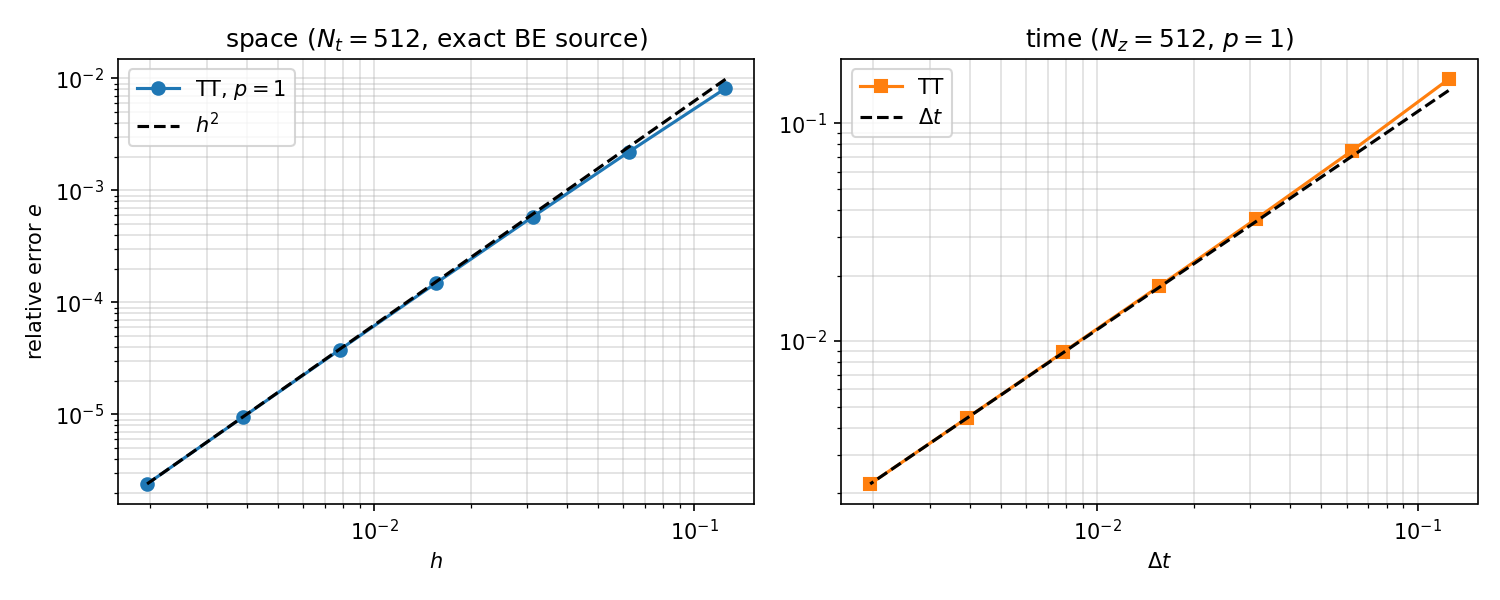
\includegraphics[width=0.95\textwidth]{convergence_mms.png}
\caption{Manufactured solution: error against $h$ (left, exact backward-difference time source) and $\Delta t$ (right), with reference slopes $h^2$ and $\Delta t$.}
\label{fig:mms}
\end{figure}

\subsection{Infinite medium: semi-analytical reference}
\label{sec:infinite}

\paragraph{Problem.} One group, isotropic scattering, $z\in\R$, lengths in mean free paths and time in collision times ($v\sigma_tt\to t$):
\begin{equation}
\big(\partial_t+\mu\,\partial_z+1\big)\psi(z,\Om,t)=\frac{c}{4\pi}\phi(z,t)+q(z,\Om,t),\qquad \phi=\int_{4\pi}\psi\,\dd\Om,
\end{equation}
with scattering ratio $c=\sigma_s/\sigma_t$, zero initial condition and the isotropic decaying Gaussian source $q=e^{-\alpha z^2}e^{-\lambda t}$.

\paragraph{Transform solution.} Laplace in $t$ ($t\to s$) and Fourier in $z$ ($\partial_z\to ik$) give $\hat\psi=\big(\frac{c}{4\pi}\hat\phi+\hat q\big)/(s+1+ik\mu)$; integrating over $\Om$ with $\int_{-1}^1\frac{\dd\mu}{a+ik\mu}=\frac2k\arctan\frac ka$ \cite{DM},
\begin{equation}
\hat\phi(k,s)=\frac{\hat q\,\mathcal T}{1-\frac{c}{4\pi}\mathcal T},\qquad
\mathcal T(k,s)=\frac{4\pi}{k}\arctan\frac{k}{s+1},\qquad
\hat q=\sqrt{\frac\pi\alpha}\,\frac{e^{-k^2/4\alpha}}{s+\lambda},
\end{equation}
so $\hat\phi=\sqrt{\pi/\alpha}\,e^{-k^2/4\alpha}(s+\lambda)^{-1}\,4\pi\arctan\frac{k}{s+1}\big/\big(k-c\arctan\frac{k}{s+1}\big)$. The rightmost singularity is at $s=c-1$ (the $k\to0$ limit of the denominator), which fixes the Bromwich abscissa.

\paragraph{Numerical inversion.} Following Ganapol \cite{Ganapol}: the Fourier inversion is written as $\phi=\frac1\pi\int_0^\infty(\mathrm{Re}\,\hat\phi\cos kz-\mathrm{Im}\,\hat\phi\sin kz)\,\dd k$, split into half-periods of the oscillation after $u=k|z|$, and the alternating series is summed with convergence acceleration. The Laplace inversion uses the Fourier cosine series $f(t)=\frac{2e^{\beta t}}{\pi}\int_0^\infty\mathrm{Re}\,F(\beta+i\omega)\cos\omega t\,\dd\omega$ \cite{DA}, again split into half-periods and accelerated with the Euler--Knopp transform, with $\beta>c-1$. Applied to the source alone, the double inversion reproduces $q(z,t)$ to $\approx10^{-5}$ (code: \code{tt\_transport.integral\_transforms.double\_inversion}).

\paragraph{TT setup.} The infinite medium is a slab of width $L=10$ with the Gaussian at $L/2$ and vacuum boundaries. Up to $T=1$ a particle travels at most one mean free path, so the boundaries see only the source tail ($e^{-\alpha\cdot25}\approx4\cdot10^{-6}$ at $\alpha=0.5$) and the slab solution equals the infinite-medium one to that level. Parameters: $\alpha=0.5$, $\lambda=0.1$, $c=0.5$ ($\sigma_{a}=0.5$, $\gamma=0$, $\Lmax=0$, $G=1$, $v=1$), $N_z=512$, $p=1$, $N_\mu=N_\varphi=256$, $N_t=1024$, $T=1$, one reconstruction point per cell; AMEn $\varepsilon=10^{-6}$, at most 20 sweeps (\code{studies/infinite\_medium/}).

\paragraph{Results.} The TT scalar flux matches the reference at all plotted times (\cref{fig:infinite}): relative $L^2$ error $5.6$, $5.2$, $4.3$ and $3.2\cdot10^{-4}$ at $t=0.10$, $0.35$, $0.60$, $0.85$, and maximum pointwise deviation $0.9$--$3.2\cdot10^{-3}$ of the peak value. The error decreases in time, as the flux grows smoother. The stored TT scalar flux over $(z,g,t)$ has ranks $[8,8]$: $1.2\cdot10^4$ entries for $5.2\cdot10^5$ values.

\begin{figure}[ht]
\centering
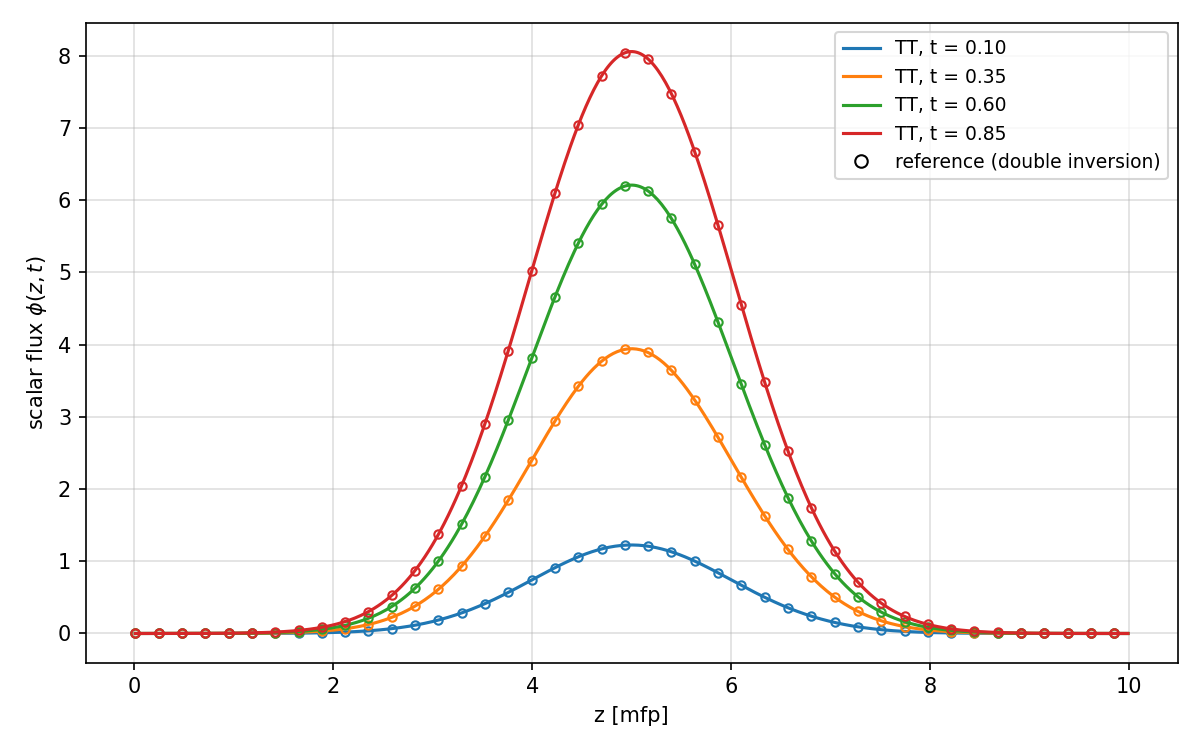
\includegraphics[width=0.8\textwidth]{infinite_medium_gaussian.png}
\caption{Infinite medium, decaying Gaussian source ($\alpha=0.5$, $\lambda=0.1$, $c=0.5$): TT scalar flux (lines) and the double-inversion reference (circles, every 12th point).}
\label{fig:infinite}
\end{figure}

\subsection{Comparison with Monte Carlo (OpenMC)}
\label{sec:mc}

Three slab problems are solved with \code{SlabTransport} and compared with OpenMC \cite{OpenMC}. Scripts, cross sections and results are in \code{studies/montecarlo/\{P0trg10, P20g128, P20g128\_het\}} (the OpenMC run directories with statepoints are not copied).

\paragraph{Common setup.} Slab $L=30$ cm, vacuum on both faces, made laterally infinite in OpenMC by reflective planes at $x,y=\pm W$, $294$ K. Source: a $2$ MeV beam along $+\hat z$ entering at $z=0$. Groups: a narrow top group $[1.9,2.1]$ MeV around the source energy, the others log-spaced down to $10^{-5}$ eV ($g=1$ the fastest).
\begin{itemize}[nosep]
\item \emph{CE run} (continuous energy): the physical reference flux on the $z$ mesh, and the multigroup cross sections tallied with \code{openmc.mgxs} \cite{MGXS}, flux-weighted over each material. The scattering moments $\sigma^l_{s,g'\to g}$ are scored with $P_l(\mu_0)$ of each analog collision.
\item \emph{MG run}: OpenMC in multigroup mode with these data, i.e.\ the same multigroup problem TT solves. To sample a cosine it tabulates the truncated series $\sum_l\frac{2l+1}{2}\sigma^lP_l(\mu)$ and clips its negative parts, so its kernel differs from the moments when the truncation oscillates.
\item \emph{TT}: the same data as MG, with the truncated series used exactly. The normal beam is not on the ordinates, so the uncollided flux $e^{-\tau(z)}$, $\tau(z)=\int_0^z\sigma_{t,1}$, is added analytically to group 1, and TT solves the collided flux with the first-collision source $Q_g=\sum_l\frac{2l+1}{4\pi}\sigma^{l}_{s,1\to g}(z)P_l(\mu)e^{-\tau(z)}$ and vacuum inflow.
\end{itemize}
TT/MG thus measures the solver error (and MG clipping), TT/CE the group-collapse and Legendre-truncation error. Fluxes are cell averages on the tally mesh, per unit incident beam intensity, $\phi_{g,i}=T_{g,i}/\Delta z$ ($T_{g,i}$ the track length per source particle in cell $i$, group $g$), independent of the transverse area. AMEn: $\varepsilon=10^{-7}$, at most 40 sweeps, kickrank 4, local systems direct up to $15000$ unknowns and GMRES otherwise, solution rounded at $10^{-8}$; DG $p=1$.

\subsubsection{Graphite, 10 groups, transport-corrected \texorpdfstring{$P_0$}{P0} (\texttt{P0trg10})}

\paragraph{Data.} Natural carbon, $1.7$ g/cm$^3$, $S(\alpha,\beta)$ table \code{c\_Graphite}. Transport correction in OpenMC's in-scatter form: $\sigma_{tr,g}=\sigma_{t,g}-\sigma_{s1,g}$ with $\sigma_{s1,g}=\sum_{g'}\sigma^1_{s,g'\to g}\phi_{g'}/\phi_g$, and the isotropic matrix $\tilde\sigma_{s0,g'\to g}=\sigma^0_{s,g'\to g}-\delta_{gg'}\sigma_{s1,g}$ (absorption unchanged). TT and MG both use $\sigma_{tr}$ as total and $\tilde\sigma_{s0}$ with $\Lmax=0$; the beam decays with $\sigma_{tr,1}$. $N_z=200$, $N_\mu=16$, $N_\varphi=3$. CE: $50\times10^5=5\cdot10^{6}$ histories; MG: $50\times5\cdot10^5=2.5\cdot10^{7}$. Median relative $1\sigma$ per cell: CE $0.07\%$ (total flux), $0.27\%$ (one group); MG $0.03\%$ and $0.13\%$. Group 10 has no flux.

\paragraph{Results.} TT and MG agree within the statistics (\cref{tab:mc-p0tr}, \cref{fig:mc-p0tr}): integrated fluxes to $0.13\%$ or better in groups 1--8, median deviation $0.5$--$1.1\sigma$, pointwise within $\approx0.3\%$ inside the slab. In the first and last cell TT is $\approx1\%$ lower in every group, where the angular flux is most anisotropic. Against CE the integrated difference is within $3\%$ in groups 1--8; pointwise it reaches $+30\%$ at the entrance in group 3, the group-collapse error of ten slab-weighted groups (MG/CE shows the same pattern). TT: operator ranks $[5,5,5,5]$, solution ranks $[33,9,9,1]$, converged in 12 sweeps ($101$ s), true residual $6\cdot10^{-7}$.

\begin{table}[ht]
\centering\small
\setlength{\tabcolsep}{4pt}
\begin{tabular}{@{}lccccccccc@{}}
\toprule
$g$ & 1 & 2 & 3 & 4 & 5 & 6 & 7 & 8 & 9 \\
\midrule
TT/MG$-1$, integrated [\%] & $0.00$ & $-0.08$ & $-0.06$ & $-0.11$ & $-0.13$ & $-0.12$ & $+0.03$ & $-0.06$ & $+0.75$ \\
median $|\phi^{\mathrm{TT}}-\phi^{\mathrm{MG}}|/\sigma_{\mathrm{MG}}$ & $0.6$ & $1.1$ & $0.7$ & $0.9$ & $1.0$ & $0.8$ & $0.8$ & $0.5$ & $0.6$ \\
TT/CE$-1$, integrated [\%] & $-0.9$ & $+2.3$ & $-1.3$ & $-2.4$ & $-2.8$ & $-2.9$ & $-2.6$ & $-2.1$ & $+9.4$ \\
\bottomrule
\end{tabular}
\caption{Graphite, 10 groups, transport-corrected $P_0$: TT versus OpenMC MG and CE. Group 9 is statistically poor ($2\%$ per cell in MG).}
\label{tab:mc-p0tr}
\end{table}

\begin{figure}[ht]
\centering
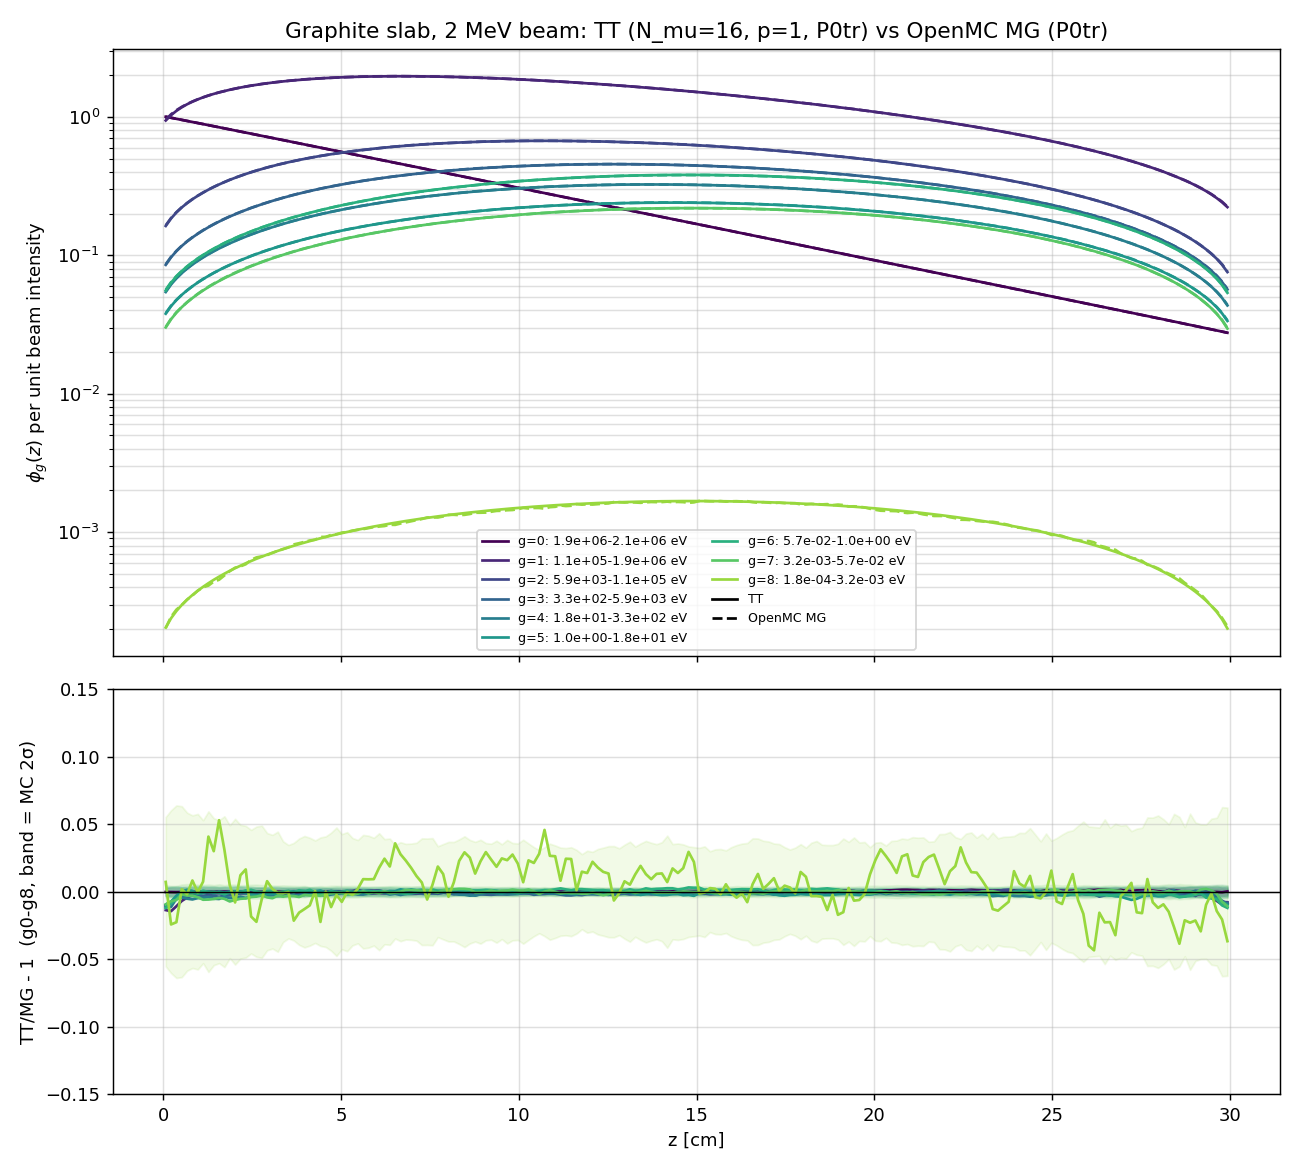
\includegraphics[width=0.75\textwidth]{mc_graphite_P0tr_g10.png}
\caption{Graphite, 10 groups, transport-corrected $P_0$. Top: scalar flux per group, TT and OpenMC MG (groups numbered from 0 in the plot). Bottom: $\phi^{\mathrm{TT}}/\phi^{\mathrm{MG}}-1$ with the MG $2\sigma$ band.}
\label{fig:mc-p0tr}
\end{figure}

\subsubsection{Graphite, 128 groups, \texorpdfstring{$P_{20}$}{P20} (\texttt{P20g128})}

\paragraph{Data.} Same material; 128 groups (the narrow top group plus 127 log-spaced groups, a factor $1.23$ in energy each) and the raw moments up to $\Lmax=20$, no transport correction. CE: $50\times5\cdot10^5=2.5\cdot10^{7}$ histories. TT is compared mainly with CE: with fine groups the collapse error is small, while the MG clipping of the box-shaped fine-group kernels affects TT/MG. An MG run with the same data ($2.5\cdot10^{7}$ histories) is shown for comparison. Median relative $1\sigma$ per cell, CE and MG alike: $0.02\%$ (total flux), $0.08\%$ (thermal band), $0.3\%$ (one group). $N_z=200$, $N_\mu=24$, azimuthal symmetry ($N_\varphi=1$).

\paragraph{Results.} TT reproduces CE to a few tenths of a percent (\cref{tab:mc-g128}, \cref{fig:mc-g128}): total flux $-0.17\%$ integrated and within $0.4\%$ pointwise up to $z=25$ cm ($-1\%$ in the last cell); per group the integrated TT/CE$-1$ is flat at $\approx-0.3\%$ from $10$ meV to $1$ MeV; global error $\|\phi^{\mathrm{TT}}-\phi^{\mathrm{CE}}\|_F/\|\phi^{\mathrm{CE}}\|_F=1.5\%$. Against MG the fast and epithermal bands agree to $0.1\%$ integrated ($0.13$--$0.14\%$ rms), but the thermal band is $+1.1\%$ throughout the slab (global error $0.36\%$): there OpenMC MG samples the clipped thermal kernels, whose truncated $P_{20}$ series are partly negative, so CE is the better reference for this case. The largest TT/CE deviation, $+21\%$ integrated, is in the group $[1.66,2.04]$ meV that contains the last Bragg edge of graphite, where the in-group kernel is a backscatter spike and the cross section jumps inside the group. TT: operator ranks $[5,25,25,5]$, solution ranks $[53,66,68,1]$ ($1.2\cdot10^5$ entries for $1.2\cdot10^6$ unknowns); AMEn stopped at the 40-sweep limit with the local GMRES stagnating near $10^{-6}$, true residual $8\cdot10^{-7}$ ($446$ s), far below the Monte Carlo noise.

\begin{table}[ht]
\centering\small
\begin{tabular}{@{}lcccccc@{}}
\toprule
TT/CE$-1$ [\%] & integrated & $z=5$ & $z=15$ & $z=25$ & $z=29.9$ & median $|z|$-score \\
\midrule
total flux $\sum_g\phi_g$ & $-0.17$ & $0.0$ & $-0.3$ & $-0.4$ & $-1.0$ & -- \\
fast ($>0.1$ MeV) & $-0.07$ & $0.0$ & $-0.2$ & $-0.2$ & $-0.8$ & $5.2$ \\
epithermal & $-0.25$ & $0.0$ & $-0.3$ & $-0.5$ & $-1.1$ & $9.0$ \\
thermal ($<1$ eV) & $-0.30$ & $-0.2$ & $-0.3$ & $-0.2$ & $-1.1$ & $3.4$ \\
\bottomrule
\end{tabular}
\caption{Graphite, 128 groups, $P_{20}$: TT versus CE, by energy band (sums over the groups inside).}
\label{tab:mc-g128}
\end{table}

\begin{figure}[ht]
\centering
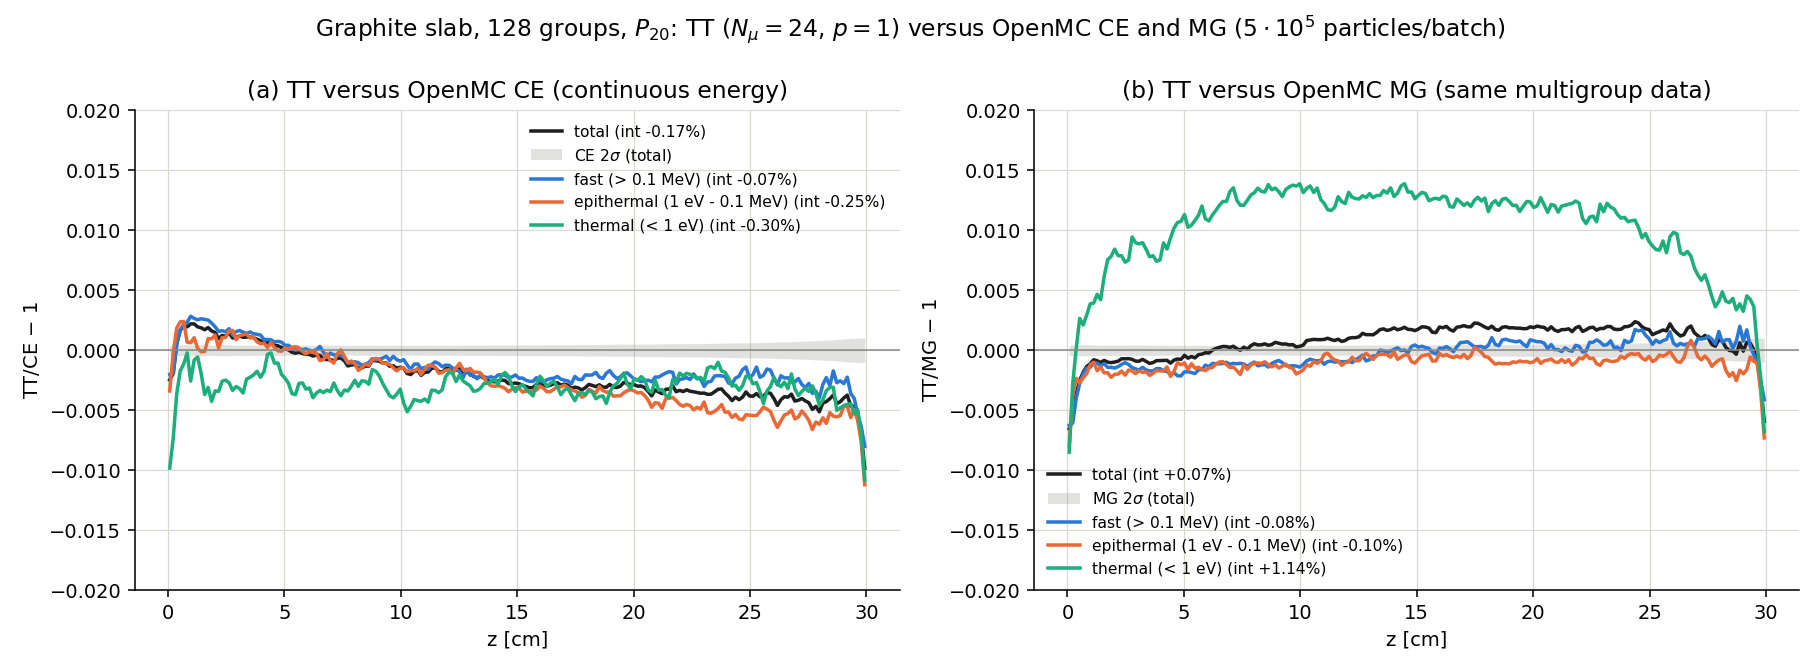
\includegraphics[width=\textwidth]{mc_graphite_P20_g128.png}
\caption{Graphite, 128 groups, $P_{20}$: TT$/$CE$-1$ (a) and TT$/$MG$-1$ (b) against depth for the total flux and three energy bands (sums of the groups inside; group mid energy as band criterion), with the $2\sigma$ band of the reference on the total.}
\label{fig:mc-g128}
\end{figure}

\subsubsection{Graphite with a \texorpdfstring{$^3$He}{He-3} detector region, 128 groups, \texorpdfstring{$P_{20}$}{P20} (\texttt{P20g128\_het})}

\paragraph{Data.} The slab of the previous case with a 2 cm region of pure $^3$He gas ($10^{-3}$ g/cm$^3$, free gas) at $z\in[14,16]$ cm: $C=2$ materials (\cref{sec:discretization}). $N_z=300$ ($h=0.1$ cm, detector faces on cell edges, same mesh as the tallies). The CE run tallies the MGXS of both materials ($50\times10^5=5\cdot10^{6}$ histories); MG uses them with the same statistics. Median relative $1\sigma$ per cell: $0.05\%$ (total flux), $0.4\%$ (thermal band), $0.9\%$ (one group); $1\sigma$ of $R$: $0.04\%$ (cells and groups treated as independent). TT takes the $2\times128$ total table, the $2\times21\times128\times128$ scattering array and the $300\times2$ region map $\chi$; the first-collision source follows $\tau(z)$ through both materials and is masked per material. With $5\cdot10^6$ histories the sub-thermal range is not sampled (zero cross sections below $\approx5\cdot10^{-4}$ eV), which affects MG and TT alike. The detector response is the He-3 absorption rate per beam neutron, $R=\sum_g\int_{\mathrm{det}}\sigma^{\mathrm{He}}_{a,g}\phi_g\,\dd z$.

\paragraph{Results.} TT reproduces MG within the statistics (\cref{tab:mc-he3}, \cref{fig:mc-he3}): global error $0.35\%$, total flux $-0.14\%$ integrated, $R^{\mathrm{TT}}=5.693\cdot10^{-2}$ against $R^{\mathrm{MG}}=5.689\cdot10^{-2}$ ($+0.07\%$; $39\%$ of it below $0.625$ eV). Against CE, $R$ agrees to $-0.20\%$ and the thermal band to $-0.8\%$. The detector depresses the flux: fast flux ($\approx1$ MeV) is $\approx20\%$ higher behind it (2 cm of moderator missing), epithermal flux drops to $0.55$ inside it, thermal flux by a factor $\approx10$ everywhere and $\approx200$ at its centre. TT: AMEn $\varepsilon=10^{-5}$, solution rounded at $10^{-6}$, kickrank 4; operator ranks $[4,45,45,1]$ (\cref{sec:operator}), solution ranks $[46,40,42,1]$, compression $0.034$; converged in 20 sweeps (final Maxres $1.0\cdot10^{-5}$), true residual $4\cdot10^{-5}$, $161$ s. The tolerance is set by the statistics: the solution error ($\lesssim10^{-4}$) is far below the MC $1\sigma$. With He-3 data collapsed directly from ENDF/B (\code{he3\_mgxs.py}) instead of tallied, $R$ changes by $+0.18\%$.

\begin{table}[ht]
\centering\small
\setlength{\tabcolsep}{3pt}
\begin{tabular}{@{}lcccccc@{}}
\toprule
 & \multicolumn{4}{c}{TT/MG$-1$ [\%]} & \multicolumn{2}{c}{TT/CE$-1$ [\%]} \\
\cmidrule(lr){2-5}\cmidrule(l){6-7}
 & integrated & He-3 cells & $z=5$ / $15$ / $25$ & median $|z|$-score & integrated & He-3 cells \\
\midrule
total flux & $-0.14$ & $+0.18$ & $-0.30$ / $+0.20$ / $-0.05$ & $3.1$ & $-0.19$ & $-0.05$ \\
fast ($>0.1$ MeV) & $-0.10$ & $+0.07$ & $-0.23$ / $+0.04$ / $-0.03$ & $1.4$ & $-0.11$ & $-0.14$ \\
epithermal & $-0.20$ & $+0.34$ & $-0.51$ / $+0.41$ / $-0.08$ & $3.0$ & $-0.26$ & $+0.08$ \\
thermal ($<1$ eV) & $-0.05$ & $-0.24$ & $-0.02$ / $-0.37$ / $+0.17$ & $0.9$ & $-0.76$ & $-0.67$ \\
He-3 absorptions $R$ & \multicolumn{4}{l}{$+0.07$} & $-0.20$ & \\
\bottomrule
\end{tabular}
\caption{Graphite with 2 cm He-3, 128 groups, $P_{20}$: TT versus OpenMC MG and CE (tallied cross sections).}
\label{tab:mc-he3}
\end{table}

\begin{figure}[ht]
\centering
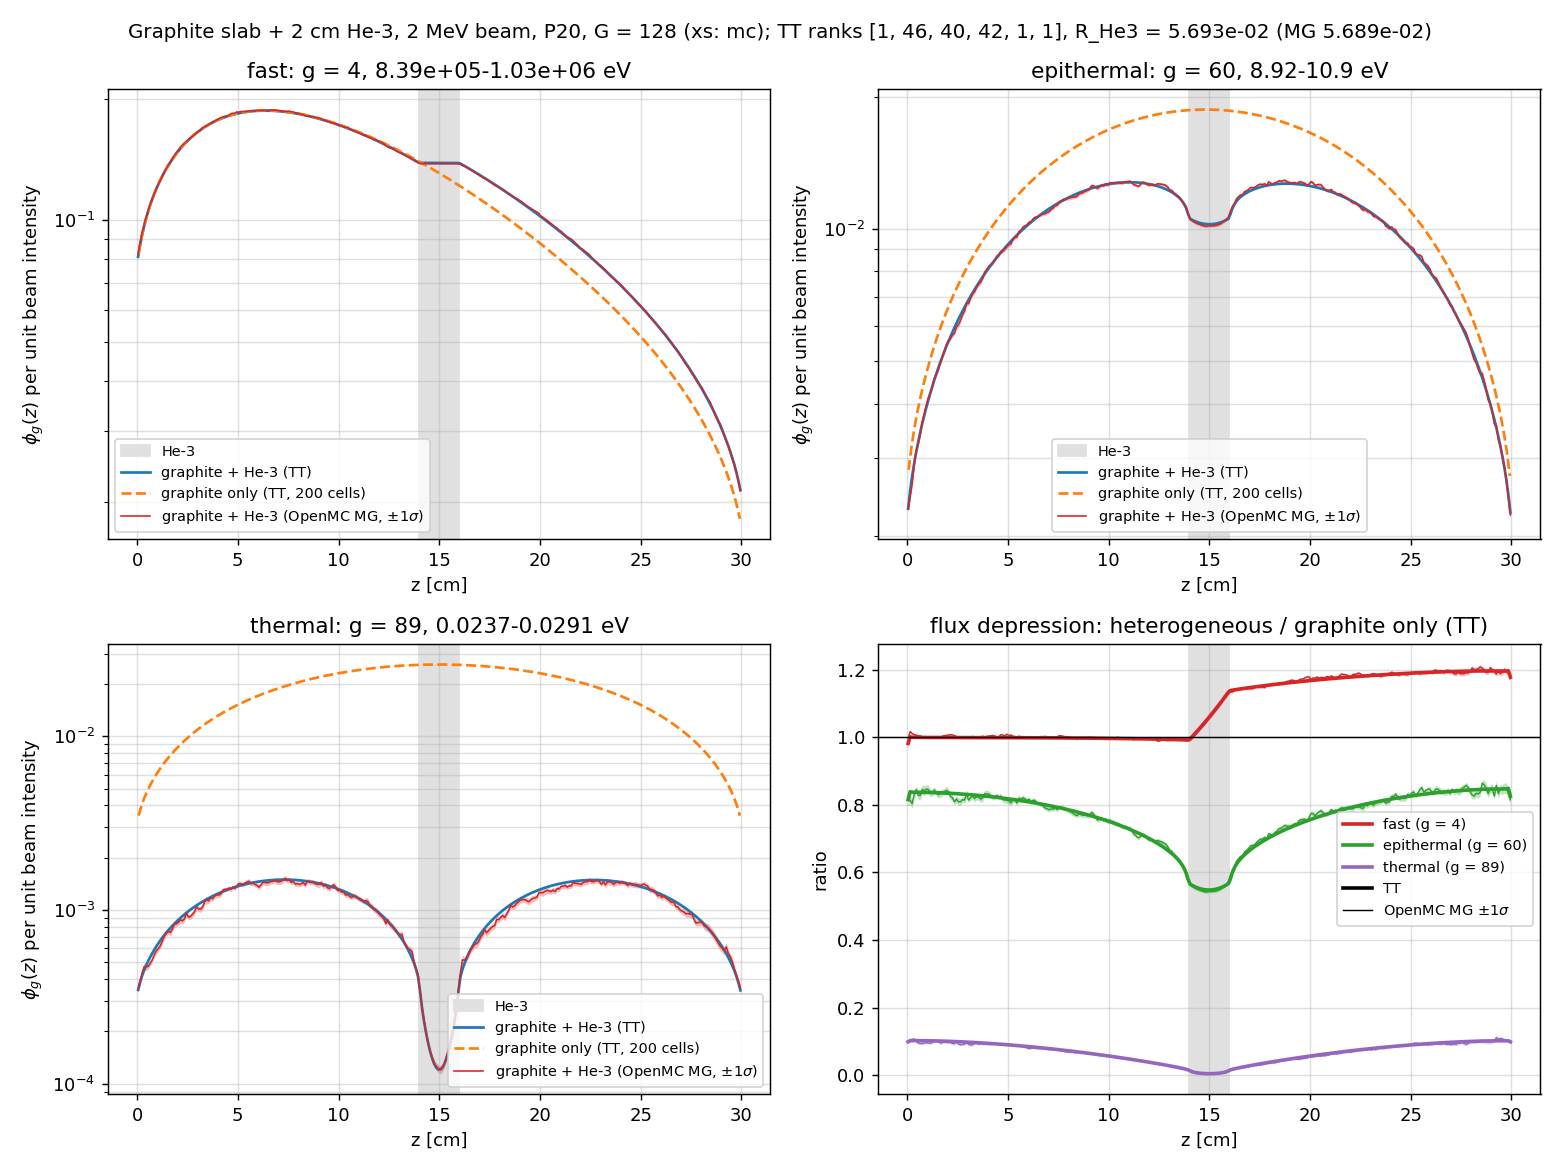
\includegraphics[width=\textwidth]{mc_graphite_he3_P20_g128.png}
\caption{Graphite with a 2 cm He-3 region (grey), 128 groups, $P_{20}$: scalar flux of a fast ($g=4$), an epithermal ($g=60$) and a thermal group ($g=89$), TT (blue), OpenMC MG with $\pm1\sigma$ (red) and the homogeneous graphite slab (TT, dashed); lower right: heterogeneous over homogeneous flux, TT (thick) and MG (thin, band).}
\label{fig:mc-he3}
\end{figure}


\FloatBarrier
\begin{thebibliography}{9}
\bibitem{ReedHill} W.~H. Reed and T.~R. Hill, Triangular mesh methods for the neutron transport equation, Los Alamos Scientific Laboratory report LA-UR-73-479 (1973).
\bibitem{Acosta} S.~Acosta, Time reversal for radiative transport with applications to inverse and control problems, \emph{Inverse Problems} 29 (2013) 085014.
\bibitem{OpenMC} P.~K. Romano, N.~E. Horelik, B.~R. Herman, A.~G. Nelson, B.~Forget, K.~Smith, OpenMC: a state-of-the-art Monte Carlo code for research and development, \emph{Ann.\ Nucl.\ Energy} 82 (2015) 90--97.
\bibitem{MGXS} W.~Boyd, A.~Nelson, P.~K. Romano, S.~Shaner, B.~Forget, K.~Smith, Multigroup cross-section generation with the OpenMC Monte Carlo particle transport code, \emph{Nucl.\ Technol.} 205 (2019) 928--944.
\bibitem{HG} L.~G. Henyey and J.~L. Greenstein, Diffuse radiation in the galaxy, \emph{Astrophys.\ J.} 93 (1941) 70--83.
\bibitem{DM} J.~J. Duderstadt and W.~R. Martin, \emph{Transport Theory}, Wiley, 1979.
\bibitem{Ganapol} B.~D. Ganapol, \emph{Analytical Benchmarks for Nuclear Engineering Applications}, OECD/NEA, 2008.
\bibitem{DA} H.~Dubner and J.~Abate, Numerical inversion of Laplace transforms by relating them to the finite Fourier cosine transform, \emph{J.\ ACM} 15 (1968) 115--123.
\end{thebibliography}

\end{document}
